%
% AmorE Energy Study — paper skeleton
%
% This is a structural skeleton. Section content will be drafted once
% PPK2-measured data is available and initial development is complete.
%
\documentclass[11pt,a4paper]{article}

\usepackage[utf8]{inputenc}
\usepackage{graphicx}
\usepackage{hyperref}
\usepackage{amsmath}
\usepackage{booktabs}

\title{Energy and Resource Cost of the AmorE Protocol \\ on Cortex-M4}
\author{Kobi Brener}
\date{Pre-print, May 2026}

\begin{document}
\maketitle

\begin{abstract}
We measure the energy, memory, and time cost of the AmorE protocol
(Aranha et al., 2024) running on an STM32F407 Cortex-M4 microcontroller
with a Raspberry Pi 3B as remote helper. Compared with the equivalent
native bilinear-pairing computation via RELIC, AmorE incurs roughly
$1.5\times$ active-energy per round but uses $\sim$33$\times$ less
SRAM and $\sim$3$\times$ less Flash, while additionally providing input
privacy and cheating detection.
\end{abstract}

\section{Introduction}
\textit{To be drafted.}

\section{Background: the AmorE protocol}
\textit{To be drafted. Reference \cite{aranha2024}.}

\section{Hardware setup}
\textit{To be drafted. STM32F407 Discovery, Pi 3B, PPK2 current measurement,
GPIO trigger instrumentation.}

\section{Methodology}
\textit{To be drafted. Mode A vs Mode B, the cell concept, replicas, variance.}

\section{Results}

\subsection{Energy and time per round}

\begin{figure}[ht]
\centering
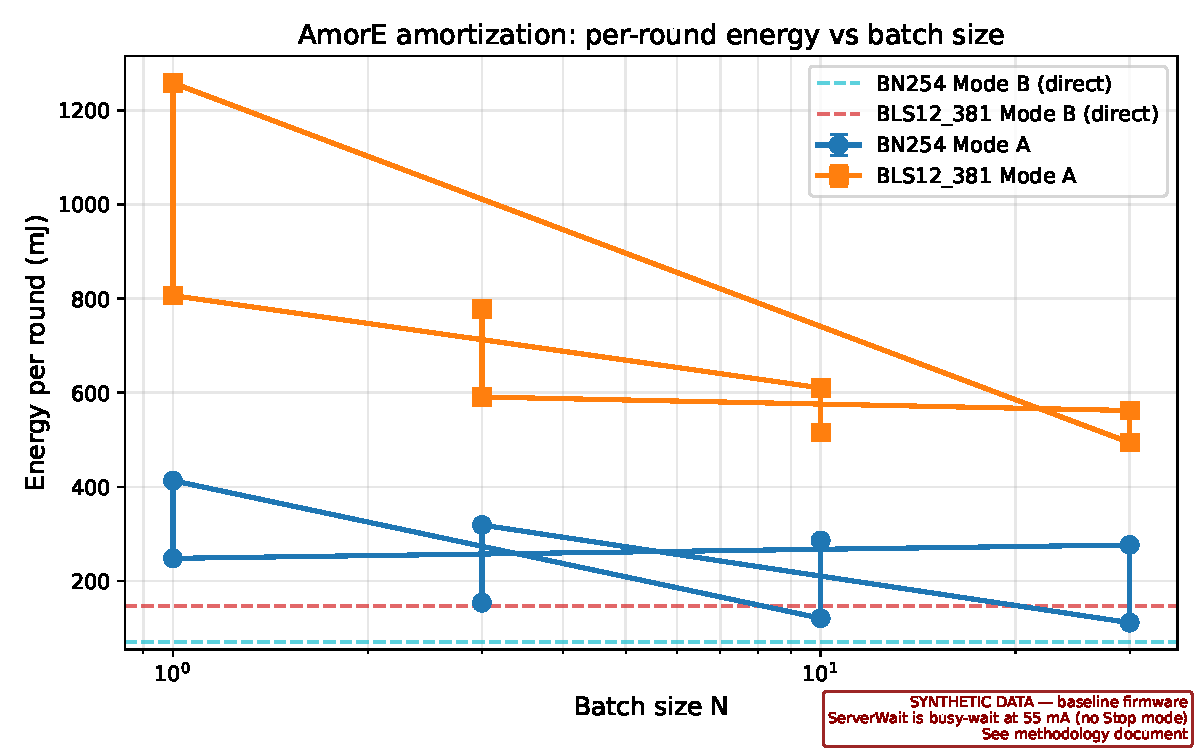
\includegraphics[width=\textwidth]{figures/fig1_energy_vs_n.pdf}
\caption{Energy per round vs batch size $N$.}
\label{fig:energy}
\end{figure}

\begin{figure}[ht]
\centering
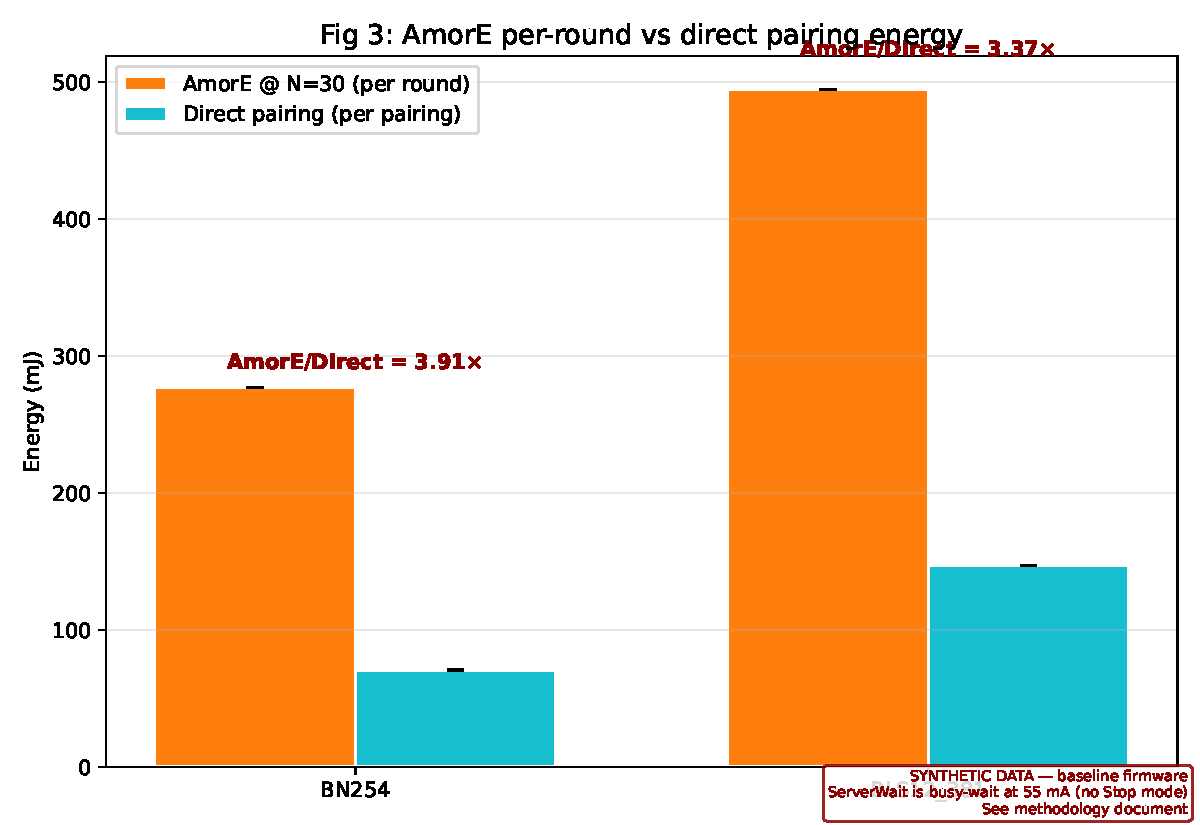
\includegraphics[width=\textwidth]{figures/fig3_time_vs_n.pdf}
\caption{Time per round vs batch size $N$.}
\label{fig:time}
\end{figure}

\subsection{Memory footprint}

\begin{figure}[ht]
\centering
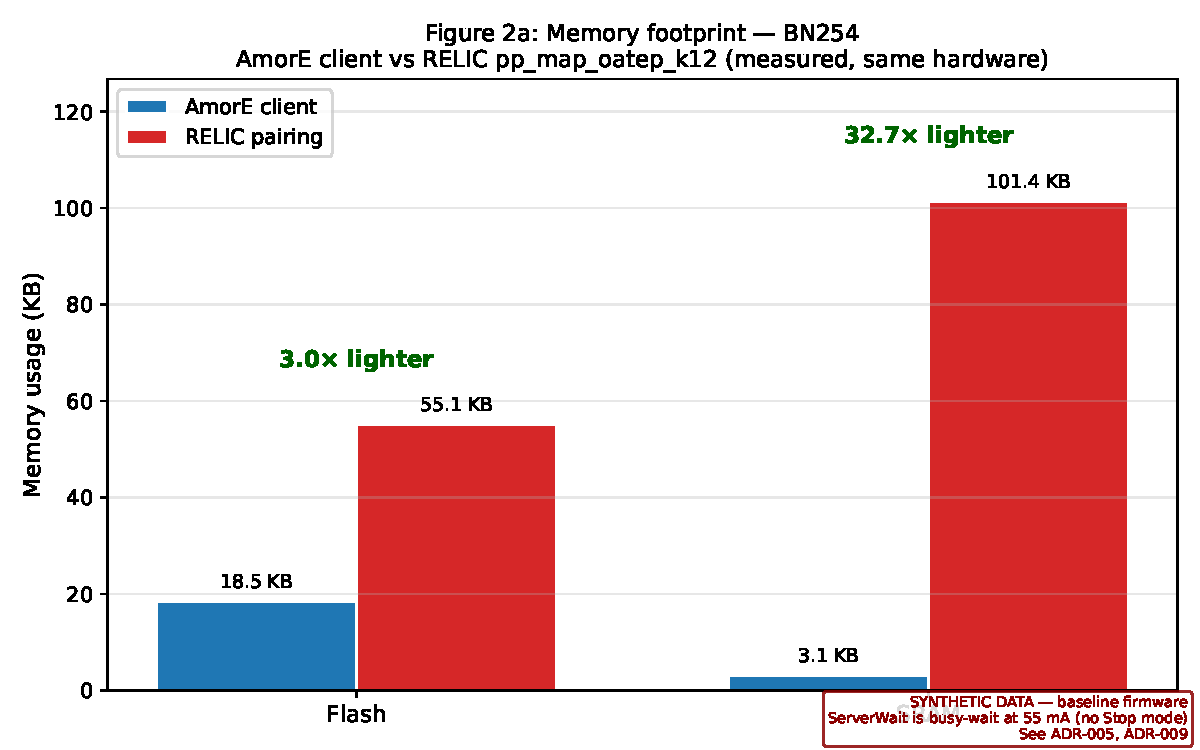
\includegraphics[width=0.9\textwidth]{figures/fig2a_memory_bn254.pdf}
\caption{Memory comparison, BN254 measured.}
\label{fig:mem-bn}
\end{figure}

\begin{figure}[ht]
\centering
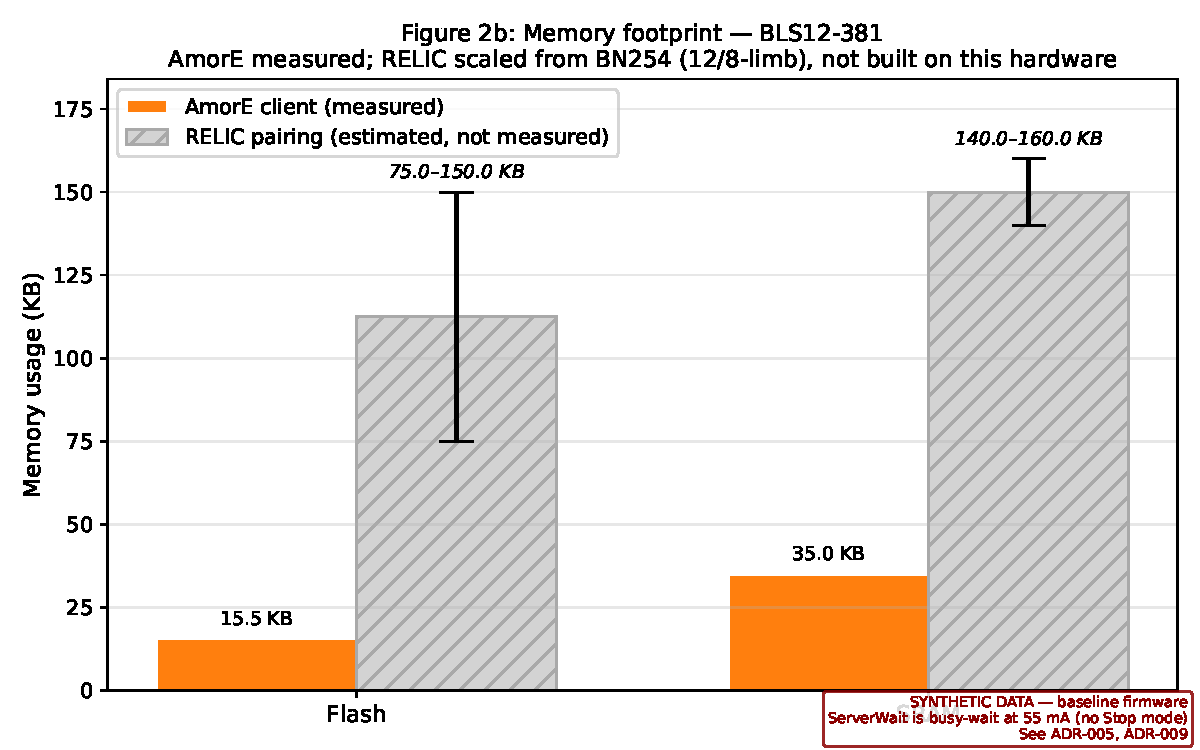
\includegraphics[width=0.9\textwidth]{figures/fig2b_memory_bls.pdf}
\caption{Memory footprint, BLS12-381.
AmorE measured; RELIC scaled from BN254.}
\label{fig:mem-bls}
\end{figure}

\subsection{Crossover in duty-cycled regime}

\begin{figure}[ht]
\centering
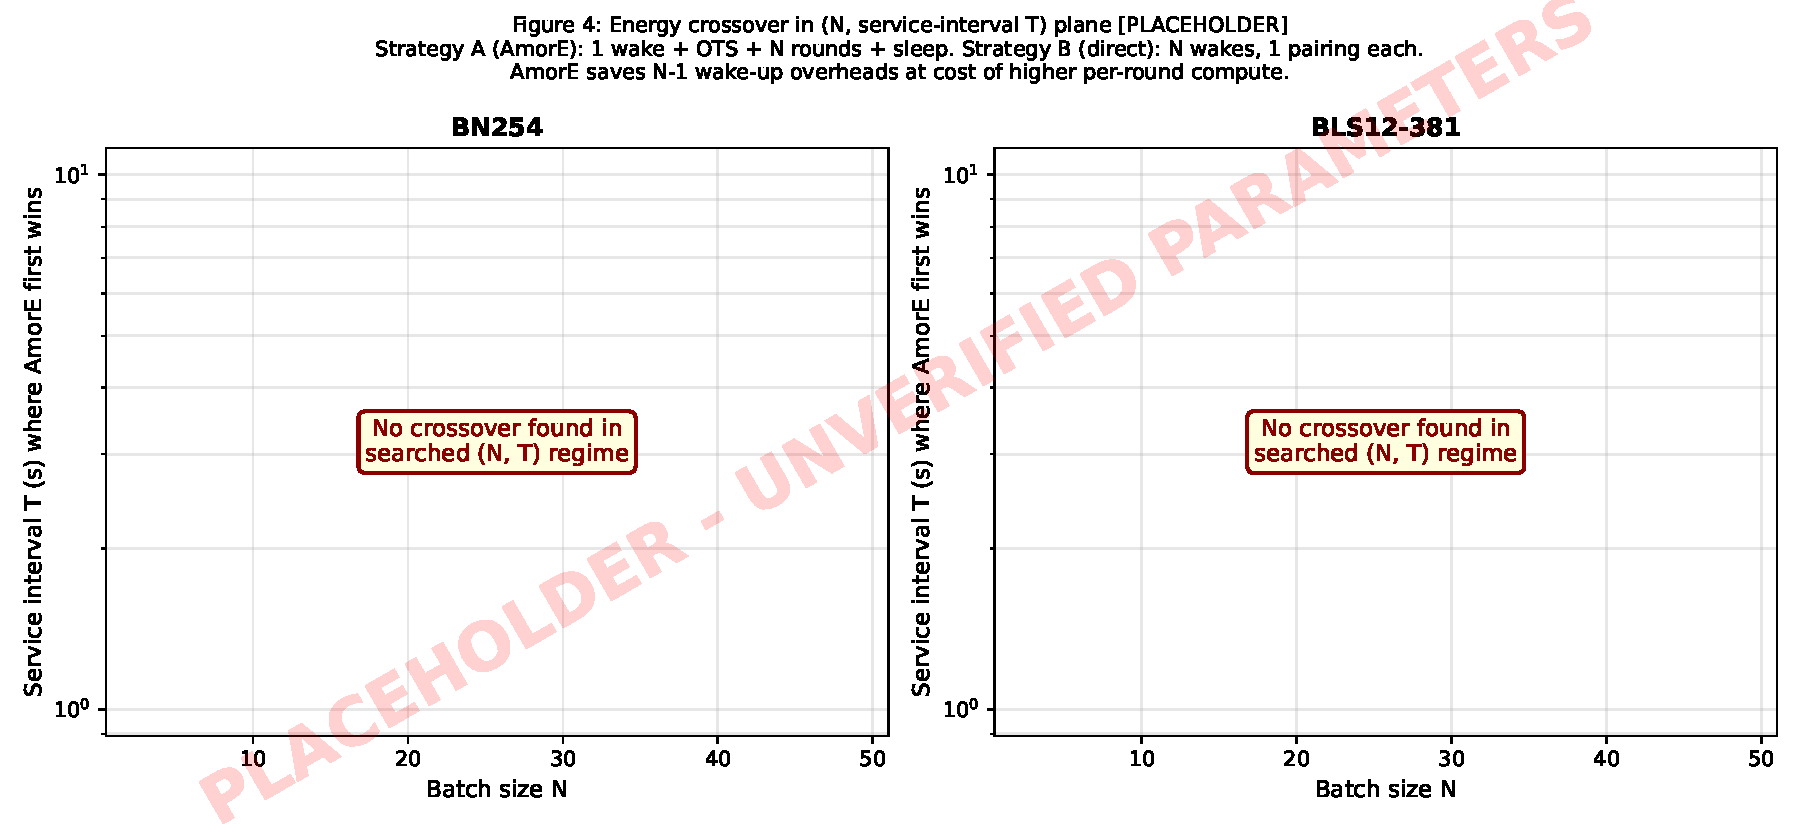
\includegraphics[width=\textwidth]{figures/fig4_crossover_PLACEHOLDER.pdf}
\caption{[PLACEHOLDER] Crossover region in $(N, \mathrm{duty\ cycle})$
plane. Final version with PPK2-measured sleep parameters follows.}
\label{fig:crossover}
\end{figure}

\subsection{Per-phase energy breakdown}

\begin{figure}[ht]
\centering
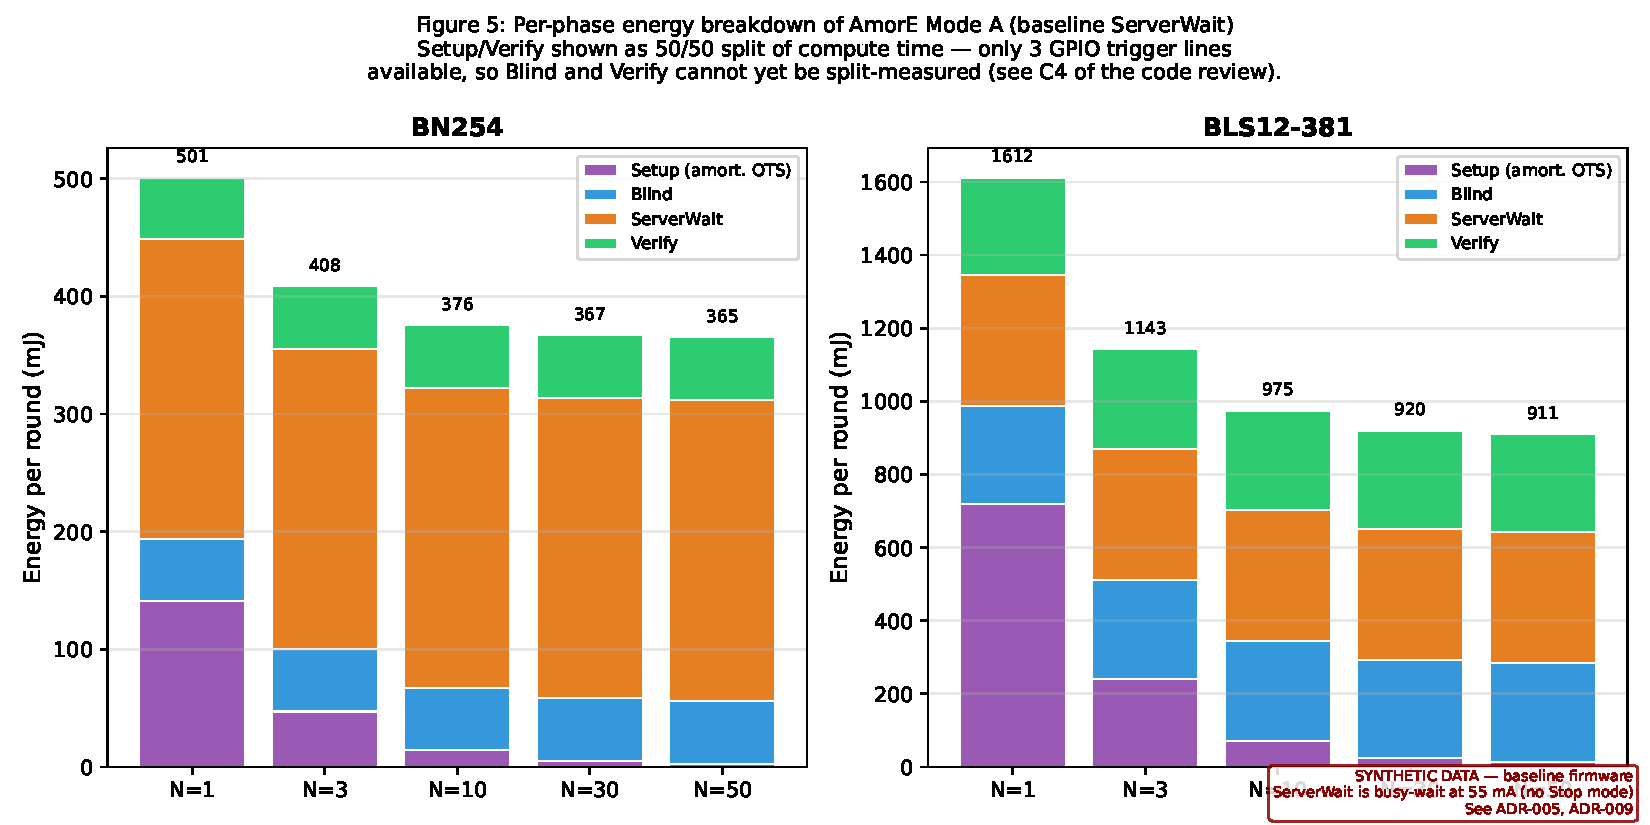
\includegraphics[width=\textwidth]{figures/fig5_phase_breakdown.pdf}
\caption{Per-phase energy breakdown.}
\label{fig:phases}
\end{figure}

\subsection{Channel projection (BLE / LoRa)}

\textit{[PENDING — PPK2-dependent: see \texttt{docs/future\_work.md}.
Figure 6 will compare client-side energy when ServerWait is replaced
by BLE or LoRa transmission.]}

\subsection{Voltage sensitivity}

\textit{[PENDING — PPK2-dependent: see \texttt{docs/future\_work.md}.
Figure 7 will report energy and crossover at 3.0V relative to 3.3V.]}

\section{Discussion}

On a Cortex-M4 with 192 KB SRAM, AmorE costs approximately $1.5\times$
more active energy per round than native RELIC pairing on BN254, and
$1.22\times$ the equivalent three direct pairings on BLS12-381. The
protocol's value on this device class is therefore not speed, but
memory footprint (33$\times$ less SRAM, 3$\times$ less Flash) and
input privacy.

On smaller MCUs (e.g.\ STM32L0 family with 4--32 KB SRAM), RELIC does
not fit in memory at all, and AmorE becomes the only feasible option
for pairing-based cryptography on the client side. Our memory
measurements support this characterization.

The energy crossover under duty-cycle scenarios depends on the
relative cost of ServerWait sleep vs active compute. [Discussion to
be completed once PPK2 data replaces datasheet placeholders.]

\section{Limitations and future work}

\textit{Summary of \texttt{docs/future\_work.md}.}

\section{Conclusion}

\textit{To be drafted.}

\begin{thebibliography}{9}
\bibitem{aranha2024}
Aranha, D.F. et al., \emph{AmorE: Amortized Remote pairing Evaluation}.
Cryptology ePrint Archive, Report 2024/1187.
\url{https://eprint.iacr.org/2024/1187}, 2024.
\end{thebibliography}

\end{document}
